\chapter{Background in scientific literature}
\label{chapter:background} 

Here is a look to the releavant papers and such - I'll update this section once
I get to work with bibtex.

This section focuses on scientific literature.

\section{Research paper open access publishing}
\label{sec:benefits_open_publishing}

Open access refers to the online literature, research data and research papers in the
context of this thesis, that are free of charge and openly available for reuse
and redistribution \cite{suber2007open}\cite{bailey2008open}. Research papers
have lived in the open access space for a much longer time and the research
shows that publishing research papers openly correlates to increased citations
(ranging between 36\% - 172\% increase \cite{DBLP:journals/corr/abs-cs-0606079},
\cite{harnad2004comparing}\cite{eysenbach2006citation}). Open access publishing of research papers make the
paper known and cited faster than non open access \cite{harnad2004comparing}.
The increase in citations to research papers is magnified in papers woth lower
ranked journals, implying that open access publishing is a cost effective way
to increase the chance of making research impact
\cite{DBLP:journals/oir/XiaN12}.

There are different ways to do open access to research papers. One division is
the Golden Road and the Green Road, where the former refers to the journals
themselves publishing with open access and the latter to so called
self-archiving, where researchers publish their papers themselves \cite{harnad2004access}.
Self-archiving can be done on the research paper's author personal website,
a disciplinary archive or a institutional repository (either an institution
wide or smaller unit, a department for example) \cite{bailey2008open}. Aalto
University has an institutional repository for research papers and theses
produced in Aalto University. It's available at \url{https://aaltodoc.aalto.fi/}.

Open access publishing is growing in popularity. A study that explored the
growth of open access publishing between years 1993-2009 reported an annual
growth rate of 18\% in open access journals and 30\% increase in open access
articles, shown in figure \ref{fig:oa_increase} \cite{laakso2011development}.
The study does not speculate on the reasons behind the growth of open access
publishing, but mentions the fact that nowadays many researchers use free
search engines such as Google Scholar (\url{https://scholar.google.fi/}) to
look for sources and that makes articles published openly to stand on equal
footing with other articles and they are more readily available. Open access
has also introduced the concept of open access mandate, which is a mandata or
a policy adopted by a university, research institution or researach funder.
The open access mandate means that the researchers working under the mandate
are rqeuired to publish their reserach papers. A list of such entities is
maintained at \url{http://roarmap.eprints.org/}. The mandate likely has
contributed to the increase in open access.

\begin{figure}
    \begin{centering}
        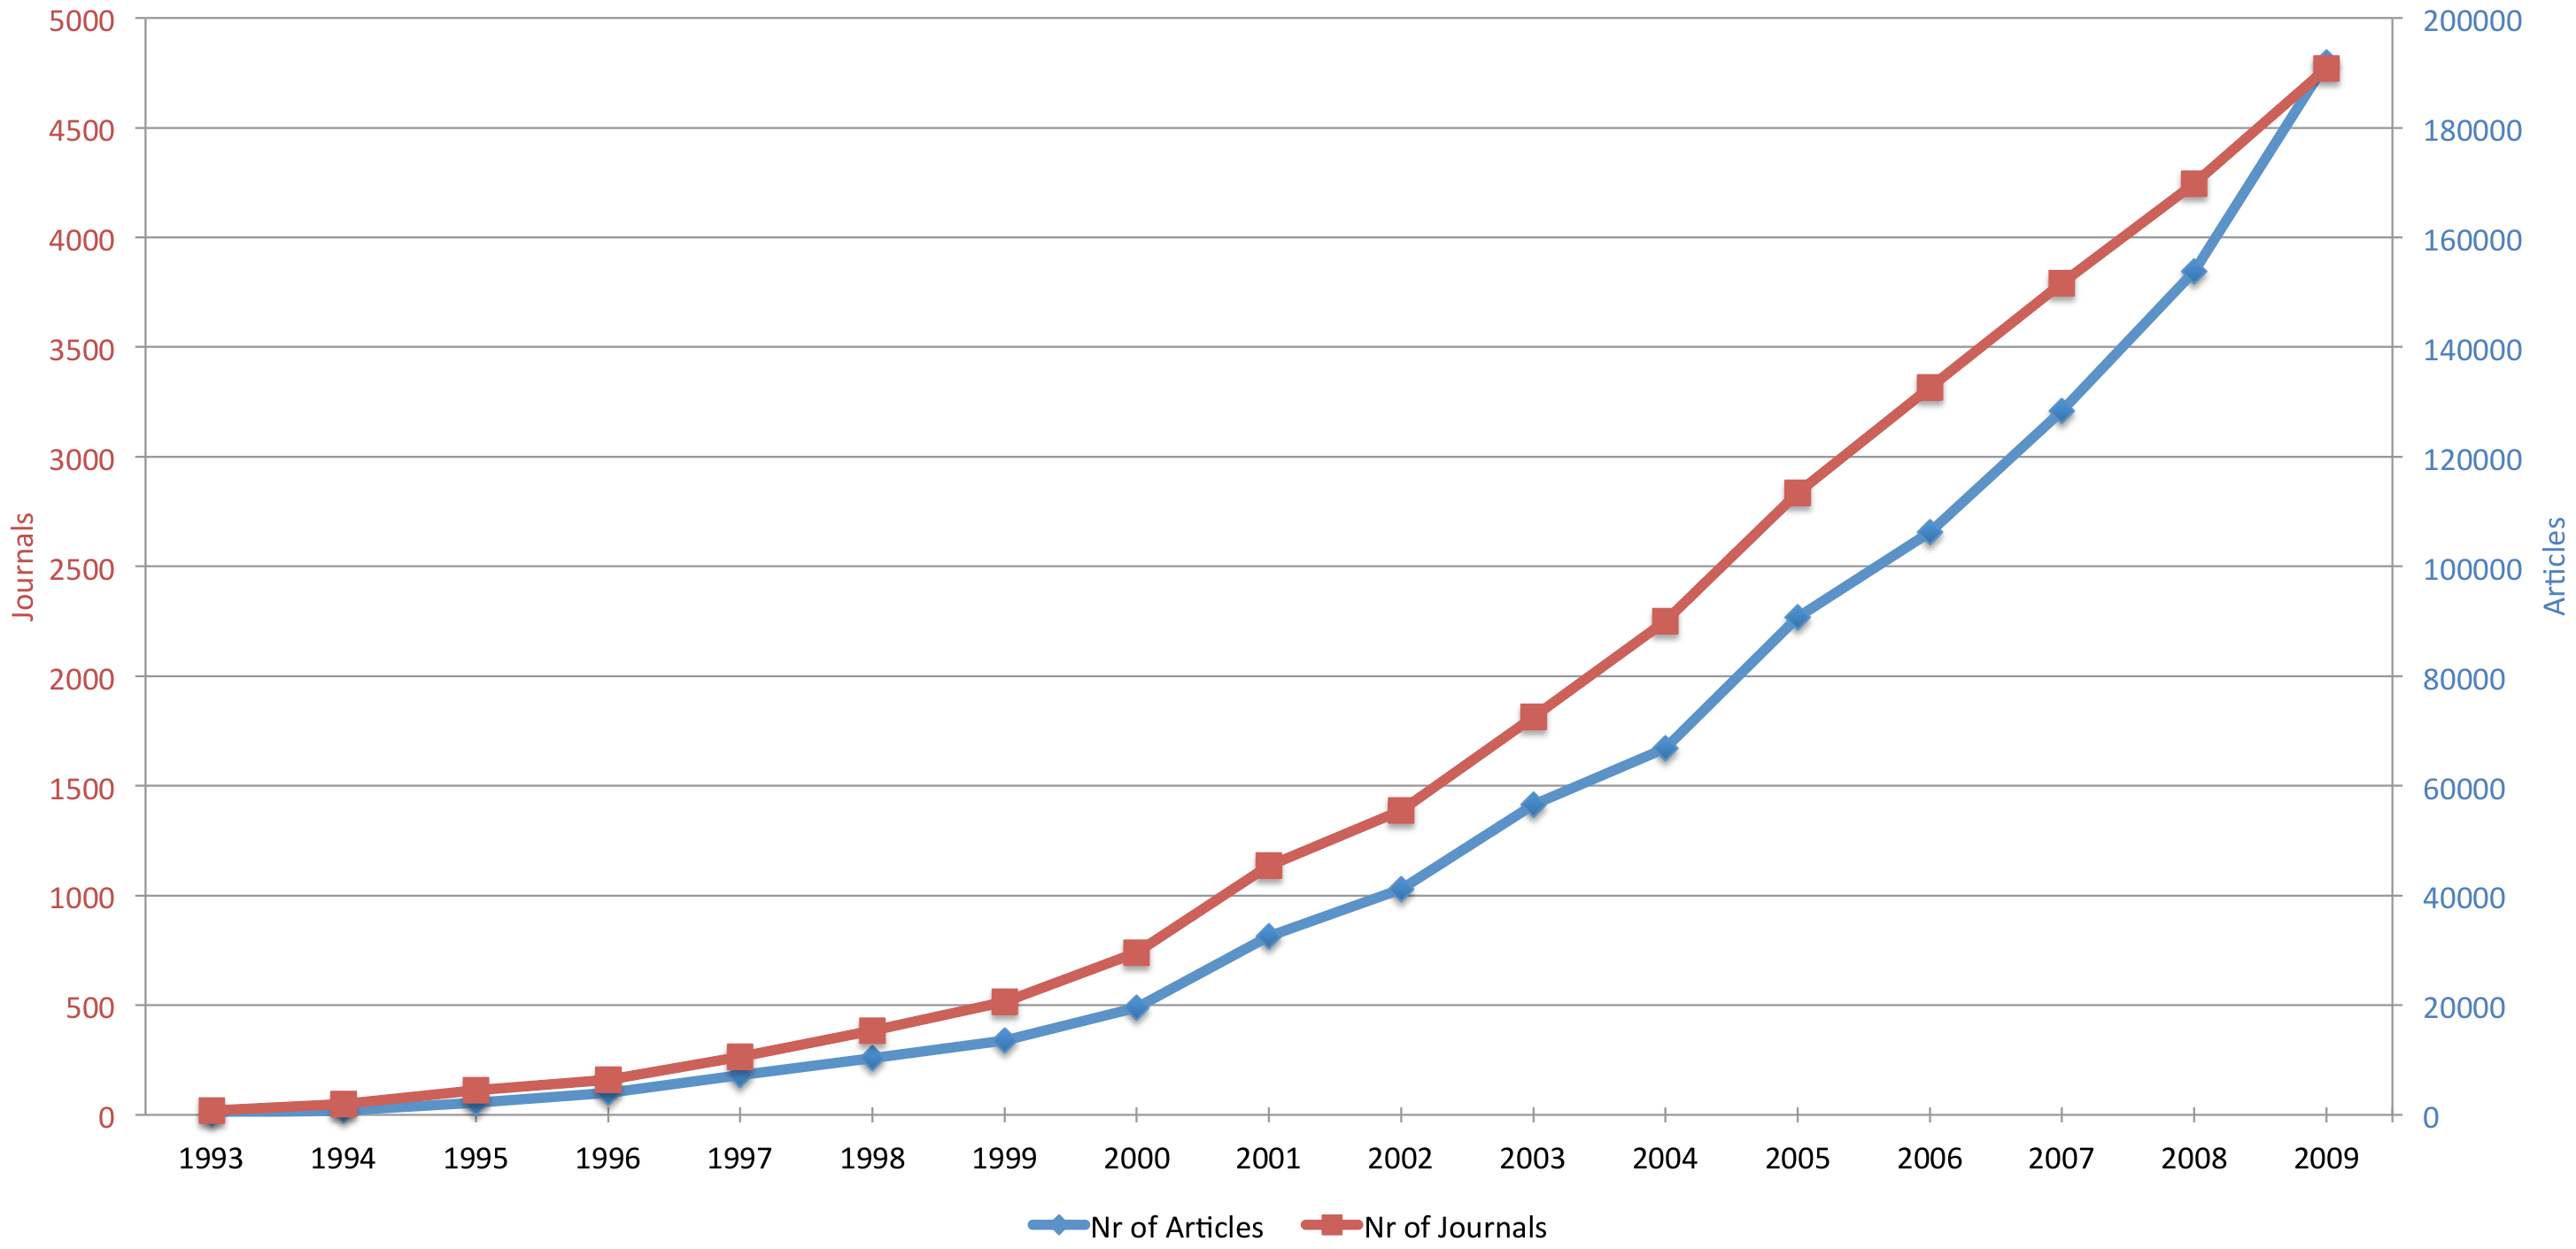
\includegraphics[width=\textwidth]{images/oa_increase}
    \end{centering}
    \caption{The growth of open access publishing between from 1993 to 2009 \cite{laakso2011development}}
    \label{fig:oa_increase}
\end{figure}

The total number of open access material is hard to estimate nowadays, but the
Directory of Open Access Journals (\url{https://doaj.org/}) measures the
amoung of open access journals world wide at 10 703 at the writing of this
thesis. The amount of open data journals and articles is growing faster than the amount
of more traditional, non open data journals \cite{laakso2011development}. This
is likely to correlate to the increased amount of open access mandates, since
mandatory open access rules imposed to the researchers correlate to a four
time increase in deposits to open access repositories
\cite{DBLP:journals/corr/SwanGHH15}.

For further reference, we can recommend the work of Stevan Harnad as a good
starting point to open access literature. He's referenced in
\cite{DBLP:journals/corr/abs-cs-0606079}, \cite{harnad2004comparing} and
\cite{harnad2004access}. If you are interested in data related to open access,
it's available botj on the Directory of Open Access Journals as well as in a
public data repository about hte growth of open access at
\url{http://dataverse.scholarsportal.info/dvn/dv/dgoa}.

\section{Research data open access publishing}
\label{sec:research_data_oa}

The idea to make research data openly accessible has been around for a long
time. As early as 1985 policies and practices to share reserach data to further
reserach and prevent fraud were developed \cite{fienberg1985sharing}.
The Internet and the emergence of data intesive science have changed the the
possibilties and quantities of research data. Research Data Alliance (RDA)
has been founded in 2013 to address the growing need of research data
publishing and sharing infrastructure \cite{DBLP:journals/dlib/BermanWW14}
\cite{DBLP:books/ms/4paradigm09}. Despite this, research data open access
publishing is far from research paper open access publishing.

Research papers should be self contained in the sense that a if you know the
area of research, you can read the research paper and understand what it was
after. Research papers often contain the processed results of the research data
behind them as well. Research data, however, is rarely self contained and
requires metadata to be useful for re use. It's also worth noting that datasets
nowadays will not be used solely by people who are experts in the fields that
the research data originated from nor will people work in geographically in the
same locations anymoer which makes metadata even more crucial for reusing the
data \cite{DBLP:journals/jbi/HarrisTTPGC09} \cite{DBLP:journals/jasis/Borgman12}.

While research papers generally follow an established structure and can easily
be published online in a PDF format, research data comes in many different
forms and flavors. For example, phylogenetic trees used in evolution
research look nothing like the brain images gathered in neuroimaging
research. This imposes a technical challenge to the solutions that
could be used to share research data - file formats are different, the
file size may be range anywhere from few hundred kilobytes to multiple
terabytes and because many fields don't share common practices on how to
manage their research data even seemingly similar datasets might be
incompatible between researchers \cite{whitlock2011data}
\cite{DBLP:journals/fini/PolineBGGHHHHKMPSAK12}.

As such, research data open access and publication is not prevalent in many
fields of science. The practices of data sharing vary a lot between fields and
even inside disciplines \cite{DBLP:journals/jasis/Borgman12}
\cite{cragin2010data}. This takes place even while all fields of science are
becoming more and more data intensive and many fields, such as psychology,
could reap great benefits from sharing research data
\cite{DBLP:books/ms/4paradigm09} \cite{wicherts2006poor}. The following
sections \ref{sec:research_data_challenges} and \ref{sec:research_data_benefits}
delve deeper into the benefits and challenges of sharing research data by
publishing it with the open access paradigm. A paper by P Arzberger et al.
\cite{DBLP:journals/datascience/ArzbergerSBBCLMUW04} summarizes these
challenges and benefits in an organizational level. A paper by Jean-Baptiste
Poline et al. describes the situation of data sharing in the field of
neuroimaging research in good depth and the discussion in the paper is also
appliccable to other fields of science
\cite{DBLP:journals/fini/PolineBGGHHHHKMPSAK12}.

\section{Challenges of sharing reserach data}
\label{sec:research_data_challenges}

Sharing research data poses many challenges, some of them organizational and
managerial while others have to do with the nature of reserach data and the
culture surrounding them. The challenges are presented in more detail below
\cite{DBLP:journals/datascience/ArzbergerSBBCLMUW04}
\cite{tenopir2011data}

\begin{itemize}
    \item Technological issues - there is a lack of infrastructure to
          effectively publish and share reserach data
    \item Institutional and managerial issues - the principles of open access
          require tailoring for insitutions, since datasets, research funding
          and similar matters require local management
    \item Financial issues - managing research data archiving and publishing
          infrastructure requires continuous financial investment beyond the
          scope of implementation and publication of the reserach projects
          results
    \item Legal and policy issues - national and international law set
          limitations to sharing research data
    \item Cultural and behavioural issues - in the end, reserach data sharing
          comes down to the actions of the researchers generating the research
          data and if the culture for it does not exist and the behaviour is
          not encouraged, there will be no sharing of research data
\end{itemize}

These issues are higlighted in the questionnaire responses in
\cite{tenopir2011data} for reasons for not making their data not accessible
to public, shown in table \ref{table:reasons_not_sharing}

\begin{table}[h]
    \centering
    \caption{Reasons for not sharing research data, questionnaire with 1329
    respondents \cite{tenopir2011data}}
    \label{table:reasons_not_sharing}
    \begin{tabular}{| l | l | l |}
      \hline
      \textbf{Reason}                           & \textbf{Responses}    & \textbf{Percent} \\
      \hline
      \rowcolor{Gray}
      Insufficient time                         & 603                   & 53.6\% \\
      \hline
      Lack of Funding                           & 445                   & 39.6\% \\
      \hline
      \rowcolor{Gray}
      Do not Have Rights ro Make Data Public    & 271                   & 24.1\% \\
      \hline
      No Place to Put Data                      & 264                   & 23.5\% \\
      \hline
      \rowcolor{Gray}
      Lack of Standards                         & 222                   & 19.8\% \\
      \hline
      Sponsor does not Require                  & 196                   & 17.4\% \\
      \hline
      \rowcolor{Gray}
      Do not Need Data                          & 169                   & 15.0\% \\
      \hline
      Other Reasons For Data Not Available      & 164                   & 14.6\% \\
      \hline
      \rowcolor{Gray}
      Should not be Available                   & 162                   & 14.4\% \\
      \hline
    \end{tabular}
\end{table}

The Tenopir paper \cite{tenopir2011data} contains many more userful tables,
showing for example, that many researchers (56.1\%) either don't know or don't have
metadata stadards for their research data and data comes in many different
categories without even going to the soecifics in the fields of science.

Research data may be serious pricavy concern especially in fields such as
genomics or healthacre related research where reserach data could be connected
to the participants of the study. There is a tension between sharing relevant
and good quality data and protecting the privacy of the participants - more
detailed data provides for a more rich research, but allows for an easier
connection on to the participants \cite{kaye2012tension}. Work is being done
to facilitate safe and accurate sharing of data with privacy concerns. Both
codes of conduct and techonoligal solutions are required, especially since the
data will outlive the participants of the study and the privacy must be
preserved for the entirety of the data's lifetime
\cite{DBLP:journals/jam/NohCJ14a} \cite{knoppers2011towards}.

A more implementation level problem to sharing research data is the fact that
due to the legal issues or maybe the desire to work on your data before
publishing it means that reserach data should be able the be shared more
locally in addition to being open to the whole world. In practice, this means
that there should be means to provide access to the research data to
collaborating researchers or people within the research organization you are
working in to enable collaboration \cite{DBLP:journals/libt/Witt08}.

\iffalse
\subsection{Research data is diverse}

While research papers generally follow a
strict structure and can easily be published in a PDF format, research data
comes in all forms and flavors. For example, research data from a brain imaging
study will look completely different from a dataset that originates from
sociological research (citation). Not only the shape of the data is different,
the size of datasets can vary from the few megabyte survey results to the
multiple petabyte simulation results from a particle collider.

Even when you get down to practicalities the diversity of research data offers
challenges - results generated from one software might be binary incompatible
with another software within one field of science. And even if you were using
the same software, our versions might be different or you might do things in
such a different way that you are not compatible with other working on the
same field.

\subsection{Research data requires metadata}

Metadata refers to data about data. It's a rescription of the data and entails
details such as when was the dataset collected, what kind of equipement was
used or if there was something noteworthy in how the experiment was run
(citation). Due to the diversity of data in different fields, the metadata
differs between fields as well (citation). Some standards for metadata exist,
but not an all fields of science (citaiton).

Research data in and on itself is the most important thing to be published, but
working on someone else's research data without the relevant metadata adds
another layer of complexity and might mean that you cannot use the data at all
(citation). One reason to publish your data is to make reproduciton of you work
(citation) easier, and without proper metadata it is hard or impossible to
do that.

\subsection{Research data might be a privacy issue}

In many fields of science (healthcare, telecommunication to name a few) the
privacy of the participants to the studies is essential. If you go about
publishing your data, you need to be concious about maintaning the anonymity
of the people taking part in your research (citation).

\subsection{Research data might be published locally}

Due to privacty issues or maybe funding issues it might be so that the data
that is used in research cannot be published to the world but maybe you can
publish it within your orgnanization or upon request. This sets access rights
requirements to your dataset, so while you might be able to openly publish
your metadata in order to tell the world that your dataset exists, your dataset
should not be available for everyone (citation). 

\subsection{Research data requires support from higher ups and related partners}

Individuals can publish their data any way they wish as long as it's within
legal boundaries. However, if institutions such as universities or librareis
wish to venture into publishing their research, individual researchers and
people working with the data need support from their organizations. Studies
have shown (citation) that organizations need to commit to the idea of open
access publishing in order for it to work.

\fi

\section{Benefits of publishing research data}
\label{sec:research_data_benefits}

When talking about the benefits of publishing and sharing reserch data two big
points are generally made. Firstly it's thought that publishing and sharing
reserach data pushes science forward by enabling more people to work on the
data and subsequently accelerate the process of making relevant discoveries.
It's also not to be forgotten that reproducibility is one of the founding
pilalrs of scientific process and reqproducing others' work without access
to their data is very hard \cite{jasny2011again}.
Secondly it's thought that the publishing of research data makes your
research papers better, giving them credibility and yielding more citations in
the process. There are more subtle benefits as well that are discussed later
in this section.

Publishing research data benefits different stakeholders involved in the
data publishing game, as shown in figure \ref{fig:beneficaries}. The figure
also lays out how the rationales of sharing research data affect the different
stakeholder groups \cite{DBLP:journals/jasis/Borgman12}.

\begin{figure}
    \begin{centering}
        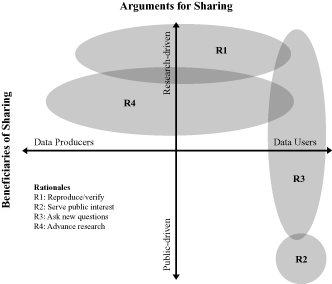
\includegraphics[width=\textwidth]{images/beneficaries}
    \end{centering}
    \caption{The different beneficiaries and rationales of data sharing \cite{DBLP:journals/jasis/Borgman12}}
    \label{fig:beneficaries}
\end{figure}

Publishing research data furthrers science by allowing new people to ask new
questions of the existing data \cite{whitlock2011data}, allowing for better
reproducability \cite{jasny2011again} and straight up widening the scope and
depth of the research in question \cite{DBLP:journals/see/FischerZ10}.
By making data publicly available the developers and people not included in the
scientific community, such as political decision makers, can also benefit from
the data being generated in the different fields of research
\cite{DBLP:journals/jasis/Borgman12}.

One can take a different view on the matter of sharing reserch data as well -
if one's results are strong and backed up by evidence, there should not be a
barrier (other than the work related to the publishing and he possible legal
issues) to publish one's data. A reason to not make data openly accessible is
the fear of reanalysis and that people might find errors in your research. This
was examined in a study in the field of psychology
\cite{wicherts2011willingness}. The findings of the study were that it was
indeed so that research papers not publishing their data had weaker results.
The comparision of amounts of errors is shown in \ref{fig:errors}. In order
to avoid this pehonemnon better policies of sharing data are needed which would
in turn make the quality of research better.

\begin{figure}
    \begin{centering}
        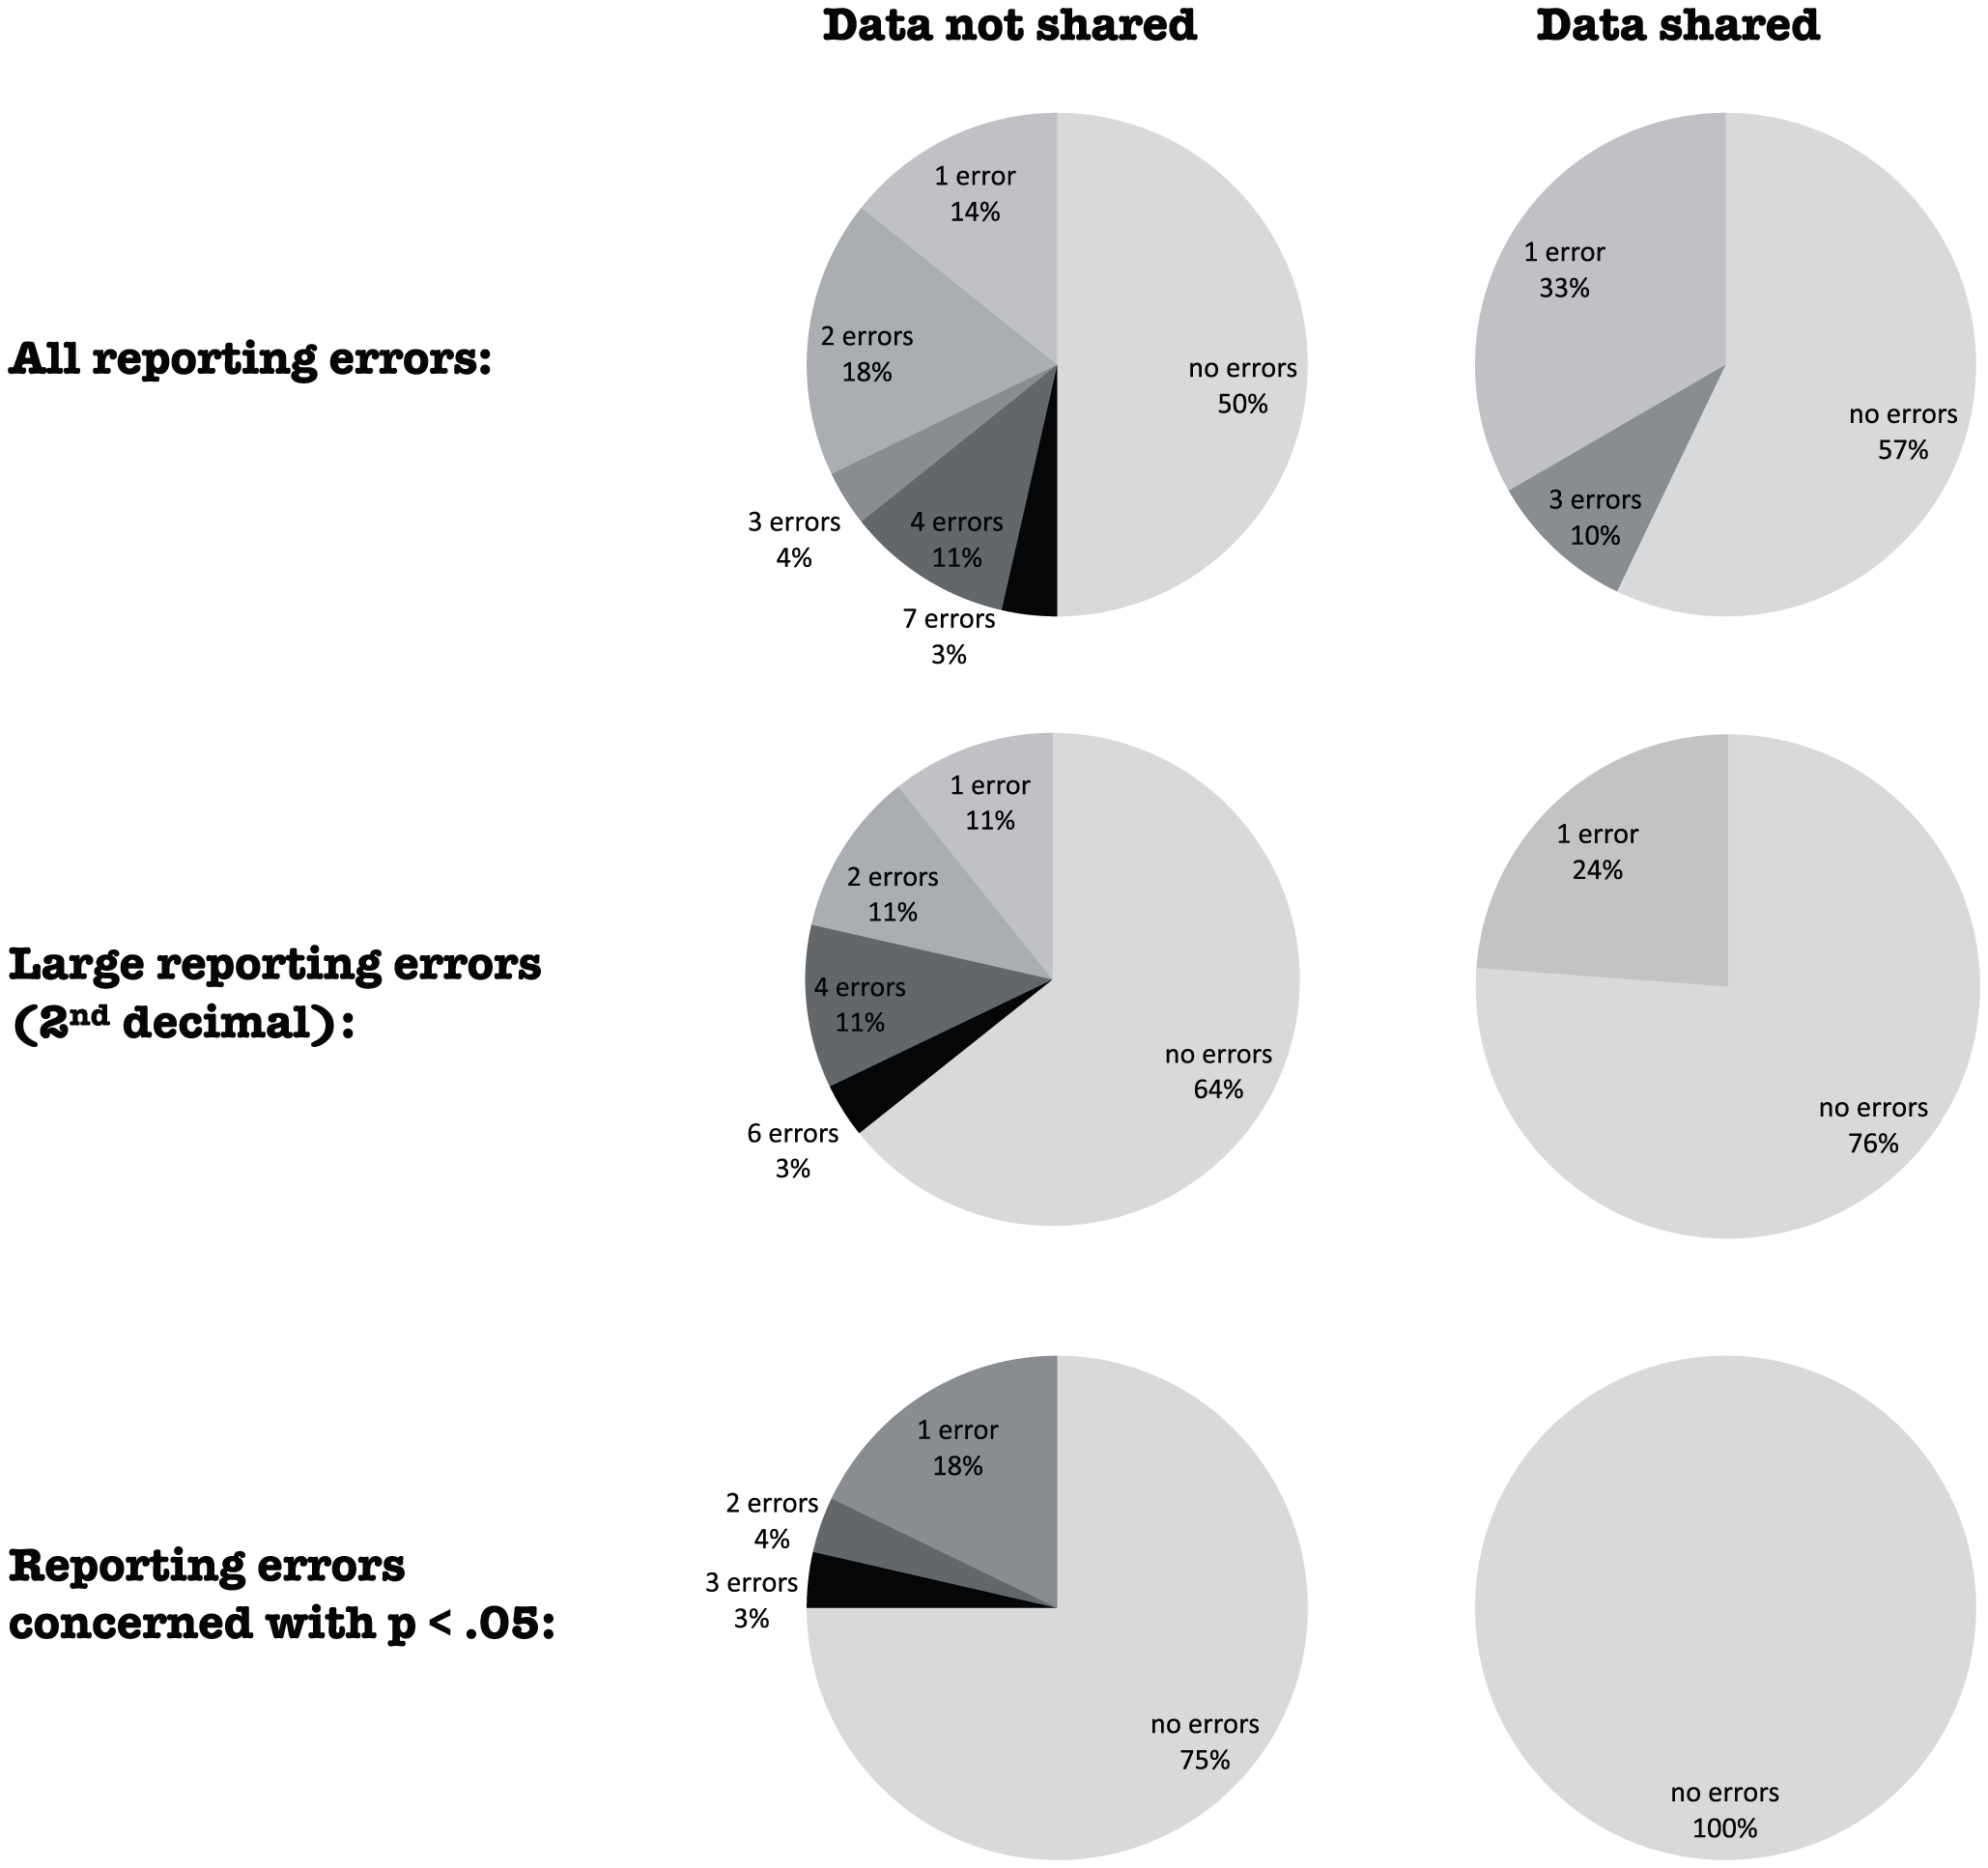
\includegraphics[width=\textwidth]{images/reporting_errors}
    \end{centering}
    \caption{The difference in reporting errors between research papers with not public and public reserch data \cite{wicherts2011willingness}}
    \label{fig:errors}
\end{figure}

In order to get research data published and openly accessible the reserachers
generating the data need to put it to the public domain. The benefits of
sharing, however, are more cler to the consumers of the published data and
preparing data for publication requires work from the person publishing the
data. Traditionally academic credit and credibility has been tied to the number
of articles published and citations of those articles and public data does not
play a role in that. However, publishing datasets can have a positive impact on
research papers' citation rate bringing the accociate credit with it
\cite{piwowar2007sharing}.

A study about cancer microarray clinical publications it was found out that
research papers that had their research data publisher received a 69\%
increase in citation rate. In the same study the 48\% of the reserach papers
that had the accociated research data included received 85\% of the aggreagate
citations \cite{piwowar2007sharing}.

In addition to providing value to the researchers publishing their papers in
the form of citations, one study \cite{piwowar2011data} study suggests that
the investment to a data repository gives a generous return of investemnt to
the insitution building and using the repository as well. The study makes a
comparision of spent money - 400 000 dollars in original reserch resulted in
16 papers, whereas the cost of running a data repository of biologigal reserach
data sets for a year would cost the same 400 000 dollars but contribute more
than 1000 papers within the following four years.

Making research data openly accessible lessens the risk of data fraud taking
place. Data fraud, which constitutes acts such as using fictitious data or
tampering with the data in order to support your conclustions, could be
prevented or made more difficult by sharing all research data. This matter is
discussed in a paper by Peter Doorn et al. \cite{DBLP:journals/ijdc/DoornDH13}
following a series of incidents where fraudulent reserch data was used as a
basis for research.

\iffalse

The benefits of research data publishing are not as straightforward as
publishing papers. Academic credit is distributed by the number of papers you
publish and by the number of citations you get to those papers. Research data
is often viewed as the fuel to the research. The actual downsides, from the
reserach, are covered in the next section (forward reference).

\subsection{Publishing reserach data yields more citations}

One of the most direct upsides of publishing reserach data is that it seems to
increase the citation count of the paper where the published data was related
to (citation). The research on this has not been done on all fields of science,
but the numbers from the fields it hase been conducted (medical science and
some others, put them down here at a later date) are impressive - up to
69\% (citation) increase in citation rates.

\subsection{Publishing research data makes your reserach reach more people}

While being quite intuitive, it's worth mentioning that open publishing of
research data results in your research being exposed to a larger audience
(citation).

\subsection{Publishing reserch data grows the impact of your research}

The impact of one's research is hard to quantify, but exposing more people to
your research and at the same time promoting your research papers enables your
research find places where it can make difference in the world (citation).
(this small section requires more meat on the bones)

\subsection{Publishing research data makes your research better quality}

The scientific principles require all scientific work to be replicateable. It
is quite hard to replicate your results just based on your paper, especially if
your paper is heavy on analysis dependant on your data (citations). In this
light publishing your research data in fact makes your research better quality.

Publishing research data should make all research data better as well. The
logic behind this is that if all research data was public, it would fall under
public scrutiny making it harder to publish fraudulent results and it would
force the authors of the data to make it more readable to the wider audience
(citation).

\subsection{Publishing research data can save you from fraud accusitions}

In addition to preventing fraud from others, if your data is public you could
easily deal with fraud accusitions by pointing people to your public data and
the analysis that was performed on that data (citation).

\section{The disadvantages of publishing research data}

There are a few strikes agains publishing research data. Some of the
disadvantages are more perceived than real, but they prevent the publication
of research data just as well.

\subsection{Preparing research data requires work}

As mentioned in section (reference backwards), publishing research data
requires metadata. Metadata entails good documentation as well as annotated
datasets and such that are not necessarily required during the research
project. Time taken away from researchers core work is a hindarance in their
daily work (citation).

This problem is made bigger by the fact that there are no best practices or
widely adopted tools to manage your data during your research process and
finally publish your data (citation).

\subsection{Publishing research data adds costs to the publication process}

Publishing is not free from the financial standpoint either. Since sicentists
are not metadata experts nor are they experts in electronic publishing, other
facets of the research institution. Open publishing of research data requires
curators for the data (for example, from a library) and adminstrators for the
system that manage the reseatch data (citation). While these groups may have
communicated in the past to some extent, publishing research data is an effort
that requires a new kind of communication and collaboration within these groups
(citation).

\fi

\section[Validity of the benefit research]{Research on the validity of increased citation rate with publishing
research data}

There is also research that suggests that the increased citation rate shown in
studies is actually a statistical artefact and that research data publication
wouldn't have a direct correlation to the increased citation rate (citations).
There are not many of these papers, but their existense suggests that there
should be more critical studies to validate the benefits of open data
publishing. On the other hand, the amount of research data being published
is quite small copmared to all data that is being generated (citation), so
when more data becomes available this kind of analysis also becomes more
valuable and accurate.

\section{Different ways of sharing research data}

Openly publishing and sharing research data takes place on different levels of
organizations. The biggest ways towards open publishing are listed below.

\begin{itemize}
    \item Institutional data repositories, discussed in \cite{cragin2010data}
    \item Disciplinary repositories, example in \cite{DBLP:journals/nar/EdgarDL03}
    \item International repositories, example in \cite{2013EGUGA..15.7202L}
    \item National repositories, example in \cite{cimino2010clinical}
\end{itemize}

A more practical look into the different implementations to these as well as
some practical benchmarking will be presened in section \ref{sec:benchmarking}

\iffalse

\subsection{Insitutional data repositories}

Notes about institutional respositories (some citations are below)

\subsection{International repositories}

Notes about international repositories (also showing some, sucg as EUDAT)

\subsection{National repositories}

Could present CSC and the national library here at this stage.

\subsection{Requirements for data sharing}

Many funding bodies require researchers to publish resedarch data in addition
to the actual papers. The research shows, however, that even though publishing
research data is required, it is not being done in practice (citation). Even
papers that are considered high impact and fields that would benefit the most
from sharing data (such as psychology) do not share their research data
(citation).

\fi

\section{Adherence to data publishing requirements}

Many funding bodies and journals require the publication of research data
related to the research papers. Adherence to this requirement has been studied
and the results are that despite the demand for sharing research data it's not
being shared commonly. In one study 10 datasets were requested from a journal
that explicitly requests sharing datasets and only one dataset was received
\cite{savage2009empirical}. In a bigger study the authors were able to gain
63 datasets out of 249 possible datasets from a journal that also requires
datasets to be shared for reanalysis \cite{wicherts2006poor}. In a study of
500 hundred papers, of which 149 were not subject to any research data
publishing requirements, only 47 papers had submitted the complete raw data
online. Of the 149 who were not required to do publish research data did not
publish anything \cite{alsheikh2011public}. The 500 hundred papers in the last
study were selected from 50 different journals by selecting the 10 research
papers with the highest impact factor.

The reasons behind not sharing data were different. In the smallest study (\cite{savage2009empirical}),
where the reserachers were able to contact the people who refused the reasons
for not sharing are listed below.

\begin{itemize}
    \item Two email addresses listed on the original research paper were no
          longer valid and once one of them was reached she was on maternity
          leave and couldn't help
    \item Two of those who didn't share didn't give a reason for not sharing - on further
          inquiry one of them responded that he was not aware of the research
          data publishing requirements
    \item One stated that he was too busy and compiling the research data
          would be too much work
    \item One had changed institutions and no longer had jurisdiction over the
          data and the people in the publishing institution responded that
          sharing would have been too much work
    \item Three did not answer the inquiry at all at first - on further inquiry
          one of them replied that he was in favor of sharing data in general
          but wanted to conduct more research on the research data himself
          first
\end{itemize}

In the biggest study the authors postulated that factors such as the 6-12
months between the publishing of the papers and the authors' investigation
the reserach data publication policies might have changed, though this is noted
to be unlikely \cite{alsheikh2011public}.

\section{Sharing Big Data}

Big Data is generally defined by the three Vs - volume, velocity and variety.
Volume refers to the amount of data - there are not usually set in stone
metrics for the volume, but as rule of thumb one should consider a warehouse
full of computers as one computing unit when it comes down to big data.
Velocity means the speed that data is being gathered. Variety in the context
of big data refers to the fact that since big data usually comes from a variety
of sources, also the content and the format of the data varies. (citations)

Nowadays big data has an added V in veracity, which means the uncertainity of
the data. In the case of big data it's impossible to tell how much of your data
is reliable, since you typically don't do validation or vetting of our data.
(citations)

All big data instances don't of course contain all of the Vs. Big Data as a
concept is rather fuzzily defined, but all big data systems contain some of the
traits described above.

In this context sharing big research data adds additional challenges, since 
you can't simply download big data research files to your computer. Some
research has gone to sharing big data datasets (cite), but since there is a lot
of work left to make "small" data sharing and management work this thesis
focuses on more traditional research data sharing.

\section{Sharing research workflows}

In addition to sharing research data, research has been done in sharing
reserch workflows. Sharing research data workflows makes replicating
experiments and sharing results even easier. Sharing workflows is common in
fields where collecting data and doing analysis are easy to automate end to
end, such as genomics (citations). This thesis does not focus sharing research
data workflows, but using making the process behind the results more visible
should make scientific work better. 

\section{Some technical examples of repository software}

\subsection{Dataverse}

\subsection{Hydra}

\subsection{CKAN}

\subsection{iRODS}

\section{Research data curation}

\section{Interesting research data related literature}

\section{General points}

Points to touch on this section:

\begin{itemize}
    \item sharing data and open publishing of results has been studied
    \item generally it's noted that sharing papers online leads to benefits
    \begin{itemize}
        \item citation rate increases
        \item impact of your research grows
        \item you reach wider audience
    \end{itemize}
    \item some research contradicts the increase in citation (comparing open
          access and closed citation), claiming that the increased citation
          rate of open access things is a statistical artefact
    \item in addition, there are papers on how you should organize your data
          sharing ways
    \item funding bodies have started demanding the publication of data
    \begin{itemize}
        \item however, people who have published in papers that require you
              to publish data don't actually do that
        \item publishing data is rare even on fields where sharing would be
              great
    \end{itemize}
    \item privacy and security is a concern
    \item present some systems available
    \item some technologies and platforms could be mentioned
    \begin{itemize}
        \item iRODS
        \item CKAN
        \item genomics sharing platforms
    \end{itemize}
    \item and then there are fringe cases related
    \begin{itemize}
        \item Adam
        \item Galaxy + Hadoop integration
    \end{itemize}
    \item notes about big data (paper about the difficulties of big data in
          research infrastructure
\end{itemize}

Article \cite{piwowar2007sharing} discusses how open data increases citation
rate.

Article \cite{howison2005ossmole} is about a collaborative repository.

Article \cite{savage2009empirical} tried requresting data from authors who were
obligated by the publisher to publish data, but 9/10 did not share data.

Article \cite{piwowar2011shares} discusses low and slowly growing publishing
rates even on fields where publishing would be most advantageous.

Article \cite{tenopir2011data} discussed the culture and perceptions of
research data publications, showing that the culture is not well developed
and organizations don't support  researchers in their long term data storing
needs.

Article \cite{whitlock2011data} discusses best practices and such and so.
Gotta read more carefully when I'm on Aalto network.

Article \cite{wicherts2006poor} shows poor availability of data even though
they should be available.

Article \cite{alsheikh2011public} shows that even high impact papers (define
high impact later) subject to data publishing requirements don't necessarily
publish stuff. Those not subjected to any policy don't publish anything.

Article \cite{piwowar2011data} promotes good ROI on publishing research data.

Article \cite{hrynaszkiewicz2010preparing} shows some guidelines for sharing
data and stuff.

Article \cite{DBLP:journals/jasis/Borgman12} tackles the conundrum of research
data.

Article \cite{DBLP:conf/isiwi/AlamMS15} discusses an easy to use platform for
sharing data.

Article \cite{DBLP:conf/jcdl/SimonGSG15} describes a video sharing tool for research
use.

Article \cite{DBLP:journals/dlib/BermanWW14} describes RDA (research data
alliance), as a entity that promotes research data sharing.

Article \cite{DBLP:journals/jam/NohCJ14a} describes a method to encrypt private
information on a public platform.

Article \cite{DBLP:conf/ACMdis/CurmiFW14a} sharing data in social media
(biometric data), read more carefully.

Article \cite{DBLP:conf/esws/EkaputraSSB14} describes and ontology based
system for sharing research data.

Article \cite{DBLP:journals/ijdc/DoornDH13} discusses whether open publishing
of data could prevent scientific fraud following a hude fraud incident.

Article \cite{DBLP:journals/ijdc/GrootveldE12} pilots the idea of a research
data peer review.

Article \cite{wicherts2011willingness} examines if not publishing research data
means that results are in fact weaker.

Book \cite{DBLP:series/synthesis/2010Rajasekar} is the iRODS primer, cite
on.

Data intensive science (the fourth paradigm), \cite{DBLP:books/ms/4paradigm09},
things to cite regarding the data science.

CKAN platform investigation, \cite{winn2013open}.

Article \cite{DBLP:journals/fini/PolineBGGHHHHKMPSAK12} talks about sharing
data in the field of brain imaging (also tackles general issued in the sharing
field).

Article \cite{knoppers2011towards} outlines code of conduct for international
data sharing in the context of genomics.

Article \cite{cragin2010data} tackles issues in insitutional and other small
institutions.

Article \cite{DBLP:journals/fgcs/RoureGS09} is about sharing scientific
workflows.

Article \cite{kaye2012tension} is about privacy issues and how to share
healthcare data in good fashion.

Classic free lunch is over (\cite{sutter2005free}), need for concurrency
increases and at the same time computing power becomes more expensive and
storage cheaper.

Article \cite{DBLP:conf/cloudcom/DemchenkoZGWL12} discusses tha challenges
of big data infrastructure in the scientific research facilities.

Article \cite{hjorland2014curating} tackles the role of libraries and data
handling professionals in the electronic world.

Executable papers as a method to reproduce data, refer to something like
this \cite{DBLP:journals/procedia/GorpM11}.

From the good old days there is this book,advocating research data sharing
before it was cool \cite{fienberg1985sharing}.

Gathering data automatically, metadata drive and so on
\cite{DBLP:journals/jbi/HarrisTTPGC09}.

Institutional repository stuff, distributed environment (university related),
here \cite{DBLP:journals/libt/Witt08}.

User engagement required in order to make data curation success with
researchers, see here \cite{DBLP:conf/ercimdl/Martinez-UribeM09}.

Overview about who shares, what, how and so on, see
\cite{borgman2010research}.

Role of libraries in emerging e-science (libraries should curate data, they are
data management experts), \cite{heidorn2011emerging}.

Good and bad things (perceptions too) about sharing research data. Medical
field, South Africa \cite{denny2015developing}.

Time is right for repositories and sharing data (data is growing, how are you
going to handle it?), see \cite{lynch2008big}.

Article \cite{eysenbach2006citation} talks about the citation advantage you get
from publishing in an open access way.

Article \cite{DBLP:journals/oir/XiaN12} talks more about getting more citations
by publishing open access style.

Article \cite{antelman2004open} is more praise towards open publishing and
research impact.

Article \cite{lawrence2001free} is an oldie, but has a lot of citations and
does talk about the merits of free online access.

Article \cite{DBLP:journals/joi/CraigPMPA07} talks about the bias of open
access - maybe it does not actually get you anywhere. Important to bring out
opposing views - it's not all rosy in the world of open access.

Article \cite{davis2008open} is another opposing voice towards the gains of
open publishing, stating that you might reach a wider audience with open
publishing but increased citation rates might be an artefact from other
sources.

Adam article \cite{DBLP:conf/sigmod/NothaftMDZLYKAH15} would be interesing from
both big data and automatic data collection. All data is data intensive
science, so making a platform to handle those aspects is interesting.

Article \cite{cimino2010clinical} speaks about a data repository implemented
by the US National Insitutes of Health where you can get health data.

Article \cite{bax2006development} presents a free meta analysis tool for health
sciences. Possibly interesting from the point of view of analyzing data
collected from multiple sources.

Article \cite{DBLP:conf/bcb/PiredduLSZ14} shows a data oriented workflow
system. Big data, genomics analysis and workflows.

As an example of repository within a field (genomics, this time), this paper
\cite{craigon2004nascarrays} shows a system to store and share data related
to this field. Another similar system here \cite{DBLP:journals/nar/EdgarDL03}.

Collaboration and sharing is presented in paper \cite{craigon2004nascarrays} in
the context of distributed open source development.

Some words about an institutional repository \cite{gibbons2009benefits}, also
quite cleanly summarizes the considerations that come in when thinking of
deploying an institutional repository.

Article \cite{DBLP:conf/icegov/SayogoP11} is yet another paper describing
the detriments to scientific data sharing.

Article \cite{irodsinproceedings} is the thing Jyväskylä wrote about the iRods
native cross GUI client.

Article \cite{DBLP:conf/elpub/Hedlund08} is about gouging the attitudes of
business people towards open publishing.

Article \cite{laakso2011development} talks about the evolution of open
publishing at the age of the internet, and points out that open publishing
is of course become more common and cheaper with internet.

Article \cite{suber2007open} is a short overview of open access publishing.

Article \cite{harnad2004comparing} boasts a bigger amount of citations to
papers that are openly accessible to the papers that are not (published in the
same journals even).

Article \cite{bailey2008open} is a nice summary about what is open access.

Article \cite{DBLP:journals/corr/abs-cs-0606079} is a longe study about OA
advantage.
